\documentclass[pdflatex,compress,mathserif]{beamer}

%\usetheme[dark,framenumber,totalframenumber]{ElektroITK}
\usetheme[darktitle,framenumber,totalframenumber]{ElektroITK}

\usepackage[utf8]{inputenc}
\usepackage[T1]{fontenc}
\usepackage{lmodern}
\usepackage[bahasai]{babel}
\usepackage{amsmath}
\usepackage{amsfonts}
\usepackage{amssymb}
\usepackage{graphicx}
\usepackage{multicol}
\usepackage{framed}
\usepackage{minted}

\definecolor{LightGray}{gray}{0.95}

\usefonttheme[onlymath]{serif}

\newcommand*{\Scale}[2][4]{\scalebox{#1}{$#2$}}%

\setbeamertemplate{caption}[numbered]

\title{METODE NUMERIK}
\subtitle{Interpolasi dan Regresi}

\author{Mifta Nur Farid}

\begin{document}

\maketitle

\section{Pengantar}

\begin{frame}{Sub-CPMK}
	Mahasiswa mampu melakukan interpolasi dan regresi (C3, P2, A2)
\end{frame}

\section{Interpolasi}

\begin{frame}{Interpolasi}
	\begin{itemize}
		\item Diketahui tabel dari pembacaan suhu dari suatu reaksi kimia
		\begin{center}
			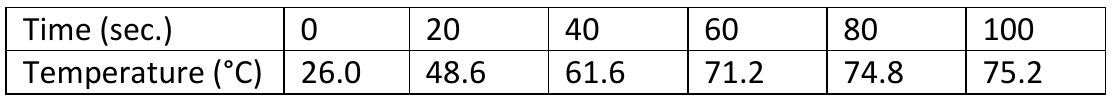
\includegraphics[width=\linewidth]{img/img01}
			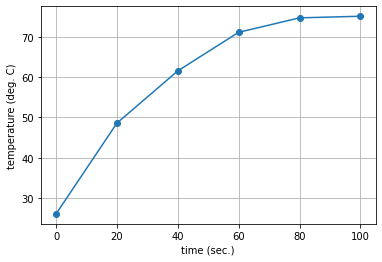
\includegraphics[width=0.7\linewidth]{img/img02}
		\end{center}
		\item Berapa suhu di 50 detik?
	\end{itemize}
\end{frame}

\subsection{Interpolasi Linear}

\begin{frame}{Interpolasi Linear}
	\begin{itemize}
		\item Metode paling mudah adalah interpolasi linear
		\begin{center}
			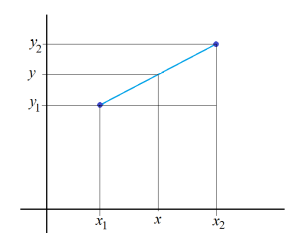
\includegraphics[width=0.5\linewidth]{img/img03}
		\end{center}
		\item Suhu $(y)$ di 50 detik $(x)$ berada di antara $(x_1, y_1)$ dan $(x_2, y_2)$, yaitu $(40, 61.6)$ dan $(60, 71.2)$
	\end{itemize}
\end{frame}

\begin{frame}{Interpolasi Linear}
	\begin{multicols}{2}
		\begin{center}
			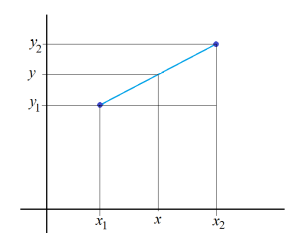
\includegraphics[width=\linewidth]{img/img03}
		\end{center}
		\columnbreak
		\begin{itemize}
			\item Persamaan garis:
			$$ \frac{y - y_1}{x - x_1} = \frac{y_2 - y_1}{x_2 - x_1}$$
			sehingga
			$$ y = y_1 + \frac{y_2 - y_1}{x_2 - x_1} (x - x_1) $$
		\end{itemize}
	\end{multicols}
\end{frame}

\begin{frame}{Interpolasi Linear}
	\begin{itemize}
		\item Sehingga suhu $(y)$ di 50 detik adalah
		$$ T_{50} = 61.6 + \frac{71.2 - 61.6}{60 - 40}(50 - 40) = 66.4~^o\text{C} $$
		\item Kekurangan: titik-titik lainnya diabaikan $\rightarrow$ interpolasi tidak bergantung pada trend kurva
		\item Metode interpolasi yang lain:
		\begin{enumerate}
			\item Interpolasi Lagrange
			\item Interpolasi Newton
		\end{enumerate}
	\end{itemize}
\end{frame}

\subsection{Interpolasi Lagrange}

\begin{frame}{Interpolasi Lagrange}
	\begin{itemize}
		\item Metode ini bergantung terhadap $n$-derajat polinomial
		\item $n$ bergantung pada jumlah titik-titik data, yaitu sebanyak $n+1$ titik
		\item Polinomial dejarat 3, $n = 3$ $\rightarrow$ jumlah titik-titik data adalah 4
		$$ y(x) = y_1l_1(x) + y_2l_2(x) + y_3l_3(x) + y_4l_4(x)$$
		atau
		$$ y(x) = \sum_{i = 1}^{n+1} y_i l_i (x) $$
	\end{itemize}
\end{frame}

\begin{frame}{Interpolasi Lagrange}
	\begin{itemize}
		\item[]
		dimana
		\begin{align*}
			l_1(x) &= \frac{(x-x_2)(x-x_3)(x-x_4)}{(x_1-x_2)(x_1-x_3)(x_1-x_4)} \\
			l_2(x) &= \frac{(x-x_1)(x-x_3)(x-x_4)}{(x_2-x_1)(x_2-x_3)(x_2-x_4)} \\
			l_3(x) &= \frac{(x-x_1)(x-x_2)(x-x_4)}{(x_3-x_1)(x_3-x_2)(x_3-x_4)} \\
			l_4(x) &= \frac{(x-x_1)(x-x_2)(x-x_3)}{(x_4-x_1)(x_4-x_2)(x_4-x_3)} \\
		\end{align*}
	\end{itemize}
\end{frame}

\begin{frame}{Interpolasi Lagrange}
	\begin{itemize}
		\item[]
		atau
		$$ l_i = \prod_{j = 1,~ j \neq i}^{n+1} \frac{(x-x_j)}{(x_i-x_j)} $$
		sehingga persamaan umum dari interpolasi Lagrange adalah
		$$ y(x) = \sum_{i=1}^{n+1} y_i \left( \prod_{j = 1,~ j \neq i}^{n+1} \frac{(x-x_j)}{(x_i-x_j)} \right) $$
	\end{itemize}
\end{frame}

\begin{frame}[fragile]{Program python interpolasi Lagrange}
	\begin{minted}[frame=lines,framesep=2mm,fontsize=\tiny,bgcolor=LightGray]{python}
x = [0, 20, 40, 60, 80, 100]
y = [26.0, 48.6, 61.6, 71.2, 74.8, 75.2]
m = len(x)
n = m-1
xp = float(input('Masukkan nilai x: '))
yp = 0

for i in range(n+1):
  L = 1
  
  for j in range(n+1):
    if j != i:
	  L *= (xp - x[j])/(x[i] - x[j])
  yp += y[i]*L
  
print('Untuk x = %.1f, y = %.1f' % (xp, yp))
	\end{minted}
\end{frame}

\subsection{Interpolasi Newton}

\begin{frame}{Interpolasi Newton}
	\begin{itemize}
		\item Interpolasi Newton juga menggunakan bentuk polinomial:
		\begin{align*}
			y(x) =&~ a_0 + (x - x_1)a_1 + (x - x_1)(x - x_2)a_2 \\
			&+ \cdots + (x - x_1)(x - x_2) \dots (x - x_n)a_n
		\end{align*}
		\item Koefisien polinomial newton didapatkan dari tabel divided difference (tabel beda terbagi)
	\end{itemize}
\end{frame}

\begin{frame}{Interpolasi Newton}
	\begin{itemize}
		\item Interpolasi Newton juga menggunakan bentuk polinomial:
		\begin{align*}
			y(x) =&~ a_0 + (x - x_1)a_1 + (x - x_1)(x - x_2)a_2 \\
			&+ \cdots + (x - x_1)(x - x_2) \dots (x - x_n)a_n
		\end{align*}
		\item Koefisien polinomial newton didapatkan dari tabel divided difference (tabel beda terbagi)
	\end{itemize}
\end{frame}

\begin{frame}{Interpolasi Newton}
	\begin{itemize}
		\item Tabel divided difference:
		\begin{center}
			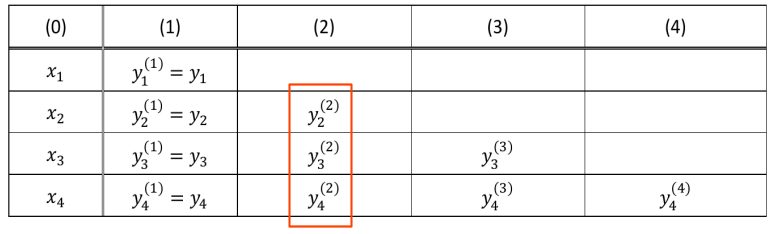
\includegraphics[width=\linewidth]{img/img04a}
		\end{center}
		\vfill
	\end{itemize}
		$$ y_i^{(2)} = \frac{y_i^{(1)} - y_1^{(1)}}{x_i - x_1},~i=2,3,4$$
\end{frame}

\begin{frame}{Interpolasi Newton}
	\begin{itemize}
		\item Tabel divided difference:
		\begin{center}
			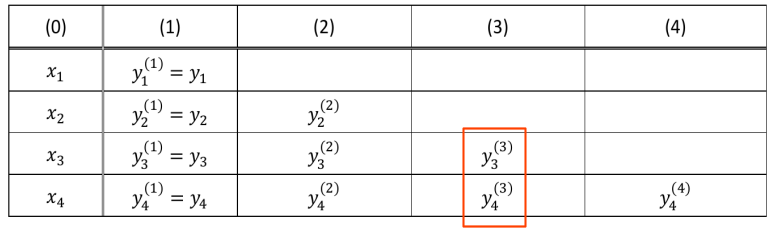
\includegraphics[width=\linewidth]{img/img04b}
		\end{center}
		\vfill
	\end{itemize}
	$$ y_i^{(3)} = \frac{y_i^{(2)} - y_2^{(2)}}{x_i - x_2},~i=3,4$$
\end{frame}

\begin{frame}{Interpolasi Newton}
	\begin{itemize}
		\item Tabel divided difference:
		\begin{center}
			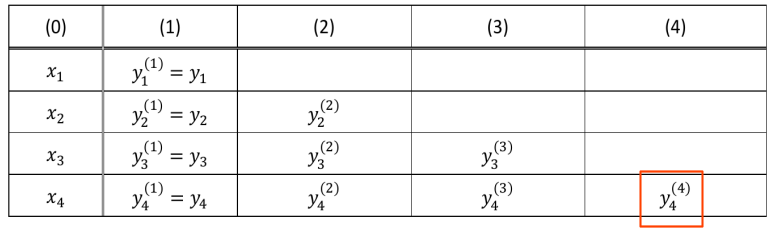
\includegraphics[width=\linewidth]{img/img04c}
		\end{center}
		\vfill
	\end{itemize}
	$$ y_4^{(4)} = \frac{y_4^{(3)} - y_3^{(3)}}{x_4 - x_3}$$
\end{frame}

\begin{frame}{Interpolasi Newton}
	\begin{itemize}
		\item Sehingga persamaan umum untuk mendapatkan tabel divided difference:
		$$ y_i^{(j+1)} = \frac{y_i^{(j)} - y_j^{(j)}}{x_i - x_j},~j=1,\dots,n \text{ dan } i=j+1,\dots,n+1$$
	\end{itemize}
\end{frame}

\begin{frame}{Interpolasi Newton}
	\begin{itemize}
		\item Koefisien polinomial newton
		\begin{align*}
			y(x) =&~ a_0 + (x - x_1)a_1 + (x - x_1)(x - x_2)a_2 \\
			&+ \cdots + (x - x_1)(x - x_2) \dots (x - x_n)a_n
		\end{align*}
		adalah
		$$a_0 = y_1^{(1)},~a_1 = y_2^{(1)},~a_2 = y_3^{(1)},\dots,a_n = y_{n+1}^{(n+1)}$$
	\end{itemize}
\end{frame}

\begin{frame}{Interpolasi Newton}
	\begin{itemize}
		\item Koefisien polinomial newton
		\begin{center}
			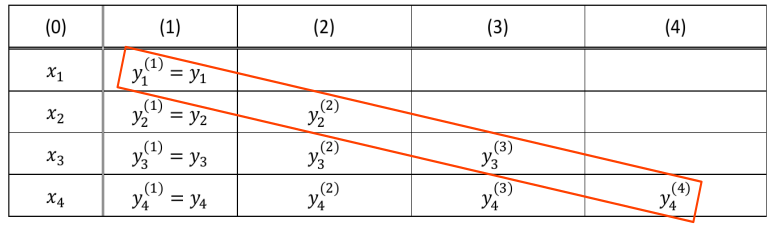
\includegraphics[width=\linewidth]{img/img04d}
		\end{center}
		$$a_0 = y_1^{(1)},~a_1 = y_2^{(1)},~a_2 = y_3^{(1)},\dots,a_n = y_{n+1}^{(n+1)}$$
	\end{itemize}
\end{frame}

\begin{frame}{Interpolasi Newton}
	\begin{itemize}
		\item persamaan umum:
		$$ y(x) = y_1^{(1)} + \sum_{i=1}^{n} \left[ \prod_{j=1}^{i}(x - x_j) \right] y_{i+1}^{(i+1)} $$
	\end{itemize}
\end{frame}

\begin{frame}[fragile]{Program python untuk interpolasi Newton}
	\begin{minted}[frame=lines,framesep=2mm,fontsize=\tiny,bgcolor=LightGray]{python}
import numpy as np

x = [0, 20, 40, 60, 80, 100]
y = [26.0, 48.6, 61.6, 71.2, 74.8, 75.2]

n = len(x) - 1
xp = float(input('Masukkan nilai x: '))
Dy = np.zeros((n+1, n+1))
Dy[:,0] = y

for j in range(n):
  for i in range(j+1, n+1):
    Dy[i,j+1] = (Dy[i,j]-Dy[j,j])/(x[i]-x[j])
    
yp = Dy[0,0]

for i in range(n):
  xprod = 1
  for j in range(i+1):
    xprod *= xp - x[j]
  yp += xprod*Dy[i+1,i+1]
 
print('Untuk x = %.1f, y = %.1f' % (xp, yp))
	\end{minted}
\end{frame}

\section{Regresi}

\begin{frame}{Regresi}
	\begin{itemize}
		\item Mencari persamaan kurva yang melalui titik-titik data
		\item Yang akan dipelajari:
		\begin{enumerate}
			\item Regresi linear
			\item Regresi non-linear
		\end{enumerate}
	\end{itemize}
\end{frame}

\subsection{Regresi Linear}

\begin{frame}{Regresi Linear}
	\begin{multicols}{2}
		\begin{center}
			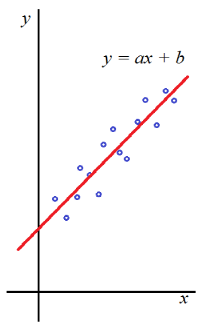
\includegraphics[width=0.6\linewidth]{img/img05}
		\end{center}
		\begin{itemize}
			\item Persamaan regresi linear:
			$$ f(x) = a + bx $$
			\item Koefisien:
			\begin{align*}
				a &= \frac{\bar{y} \sum x_i^2 - \bar{x}\sum x_i y_i}{\sum x_i^2 - n\bar{x}^2} \\
				b &= \frac{\sum x_i y_i - \bar{x} \sum y_i}{\sum x_i^2 - n\bar{x}^2}
			\end{align*}
			\item $\bar{x}$ dan $\bar{y}$ adalah nilai rata-rata
			$$ \bar{x} = \frac{1}{n} \sum_{i=1}^{n} x_i \text{ dan } \bar{y} = \frac{1}{n} \sum_{i=1}^n y_i$$
		\end{itemize}
	\end{multicols}
\end{frame}

\subsection{Regresi Non-linear}

\begin{frame}{Regresi Non-linear}

\end{frame}

\end{document}
